\section{Il progetto}

\subsection{Formazione e descrizione di Nuovo Sportello}
Nel primo periodo c'è stato naturalmente un periodo di formazione, svolto in presenza nella sede di Padova di Lynx. Durante le ore di formazione, il tutor \NST mi ha presentato l'architettura di Sportello in ogni sua parte, con le tecnologie utilizzate. Ho avuto modo di entrare in contatto per la prima volta con un sistema molto complesso e di vederne la sua evoluzione nel tempo. \\

\begin{figure}[h]
	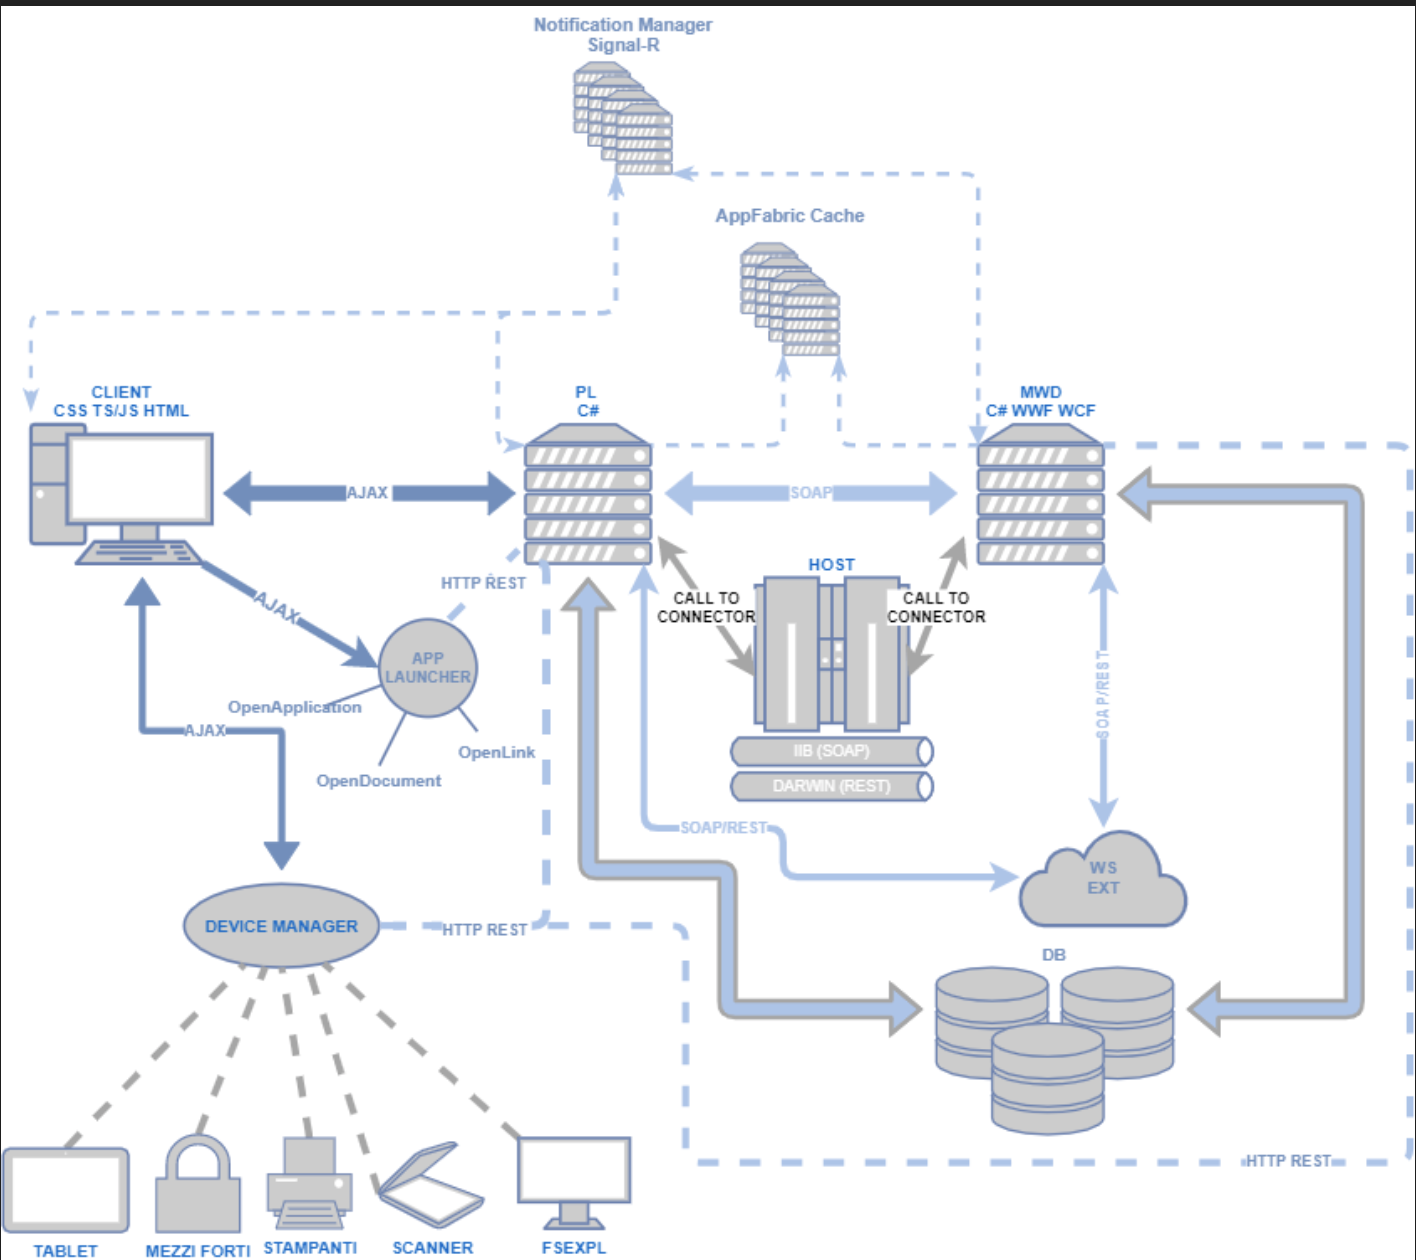
\includegraphics[width=\textwidth]{./res/img/infrastruttura sportello.png}
    \caption{Overview dell'infrastruttura di Sportello}
\end{figure}

Com'è possibile vedere dalla figura la parte front-end dell'infrastruttura a sinistra è basata su ASP.NET. Il client scritto in Typescript e HTML comunica tramite chiamate Ajax con un server chiamato Presentation Layer scritto in C\#, il quale contiene tutta la logica complessa e ha la possibilità di eseguire chiamate ai server di Intesa SanPaolo o a collegarsi a servizi Middleware. Questa parte è responsabile anche del collegamento a device fisici controllabili via software. \\
Nel back-end ho già nominato i server Middleware che si occupano di esporre servizi basati su protocolli di tipo SOAP. In questo frangente sono venuto a contatto con una tecnologia Microsoft: \textit{WCF}. Windows Communication Foundation (WCF) è un framework per costruire servizi in modo sicuro ed è efficiente. È utilizzata anche una versione Event Driven con una programmazione grafica, attraverso file .xaml, chiamata Windows Workflow Foundation. \\
Sempre a back-end sono disponibili tutti i DB basati su Microsoft SQL Server e l'host di Intesa SanPaolo, server contente tutti i dati della banca. \\

\subsubsection{ASP.NET}
ASP.NET è un framework creato da Microsoft per lo sviluppo di web application. Segue il pattern MVC (Model View Controller), ripreso poi dall'infrastruttura front end di Sportello. La view è costruita attraverso le normali tecnologie web, mentre il model e il controller sono scritti in C\#. I model non sono nient'altro che \textit{contract} che vengono utilizzati nel comunicazioni Ajax tra le componenti. I controller espongono metodi utili al front end implementandone la logica di fondo.  

\subsubsection{SOAP}
Durante la prima fase del tirocinio mi è stato molto utile il concetto di chiamata SOAP. Simple Object Access Protocol è utilizzato per scambiare informazioni strutturate basato principalmente su HTTP. SOAP utilizza un sistema di incapsulamento delle informazioni e anche per questo è portato per il trasporto di oggetti.

\subsection{Strumenti utilizzati}

\subsubsection{Visual Studio 2013/2017}
\begin{figure}[h]
	
\includegraphics[width=0.2\textwidth]{./res/img/visual-studio-2013-logo.png}
    \caption{Logo di Visual Studio}
\end{figure}